\documentclass{standalone}
\usepackage{tkz-fct}
\usepackage{tkz-euclide}
\usepackage{amsmath}
\usepackage{color}
\renewcommand*\familydefault{\sfdefault}
\usepackage{sansmath}
\sansmath
\definecolor{gray75}{gray}{0.75}
\begin{document}
 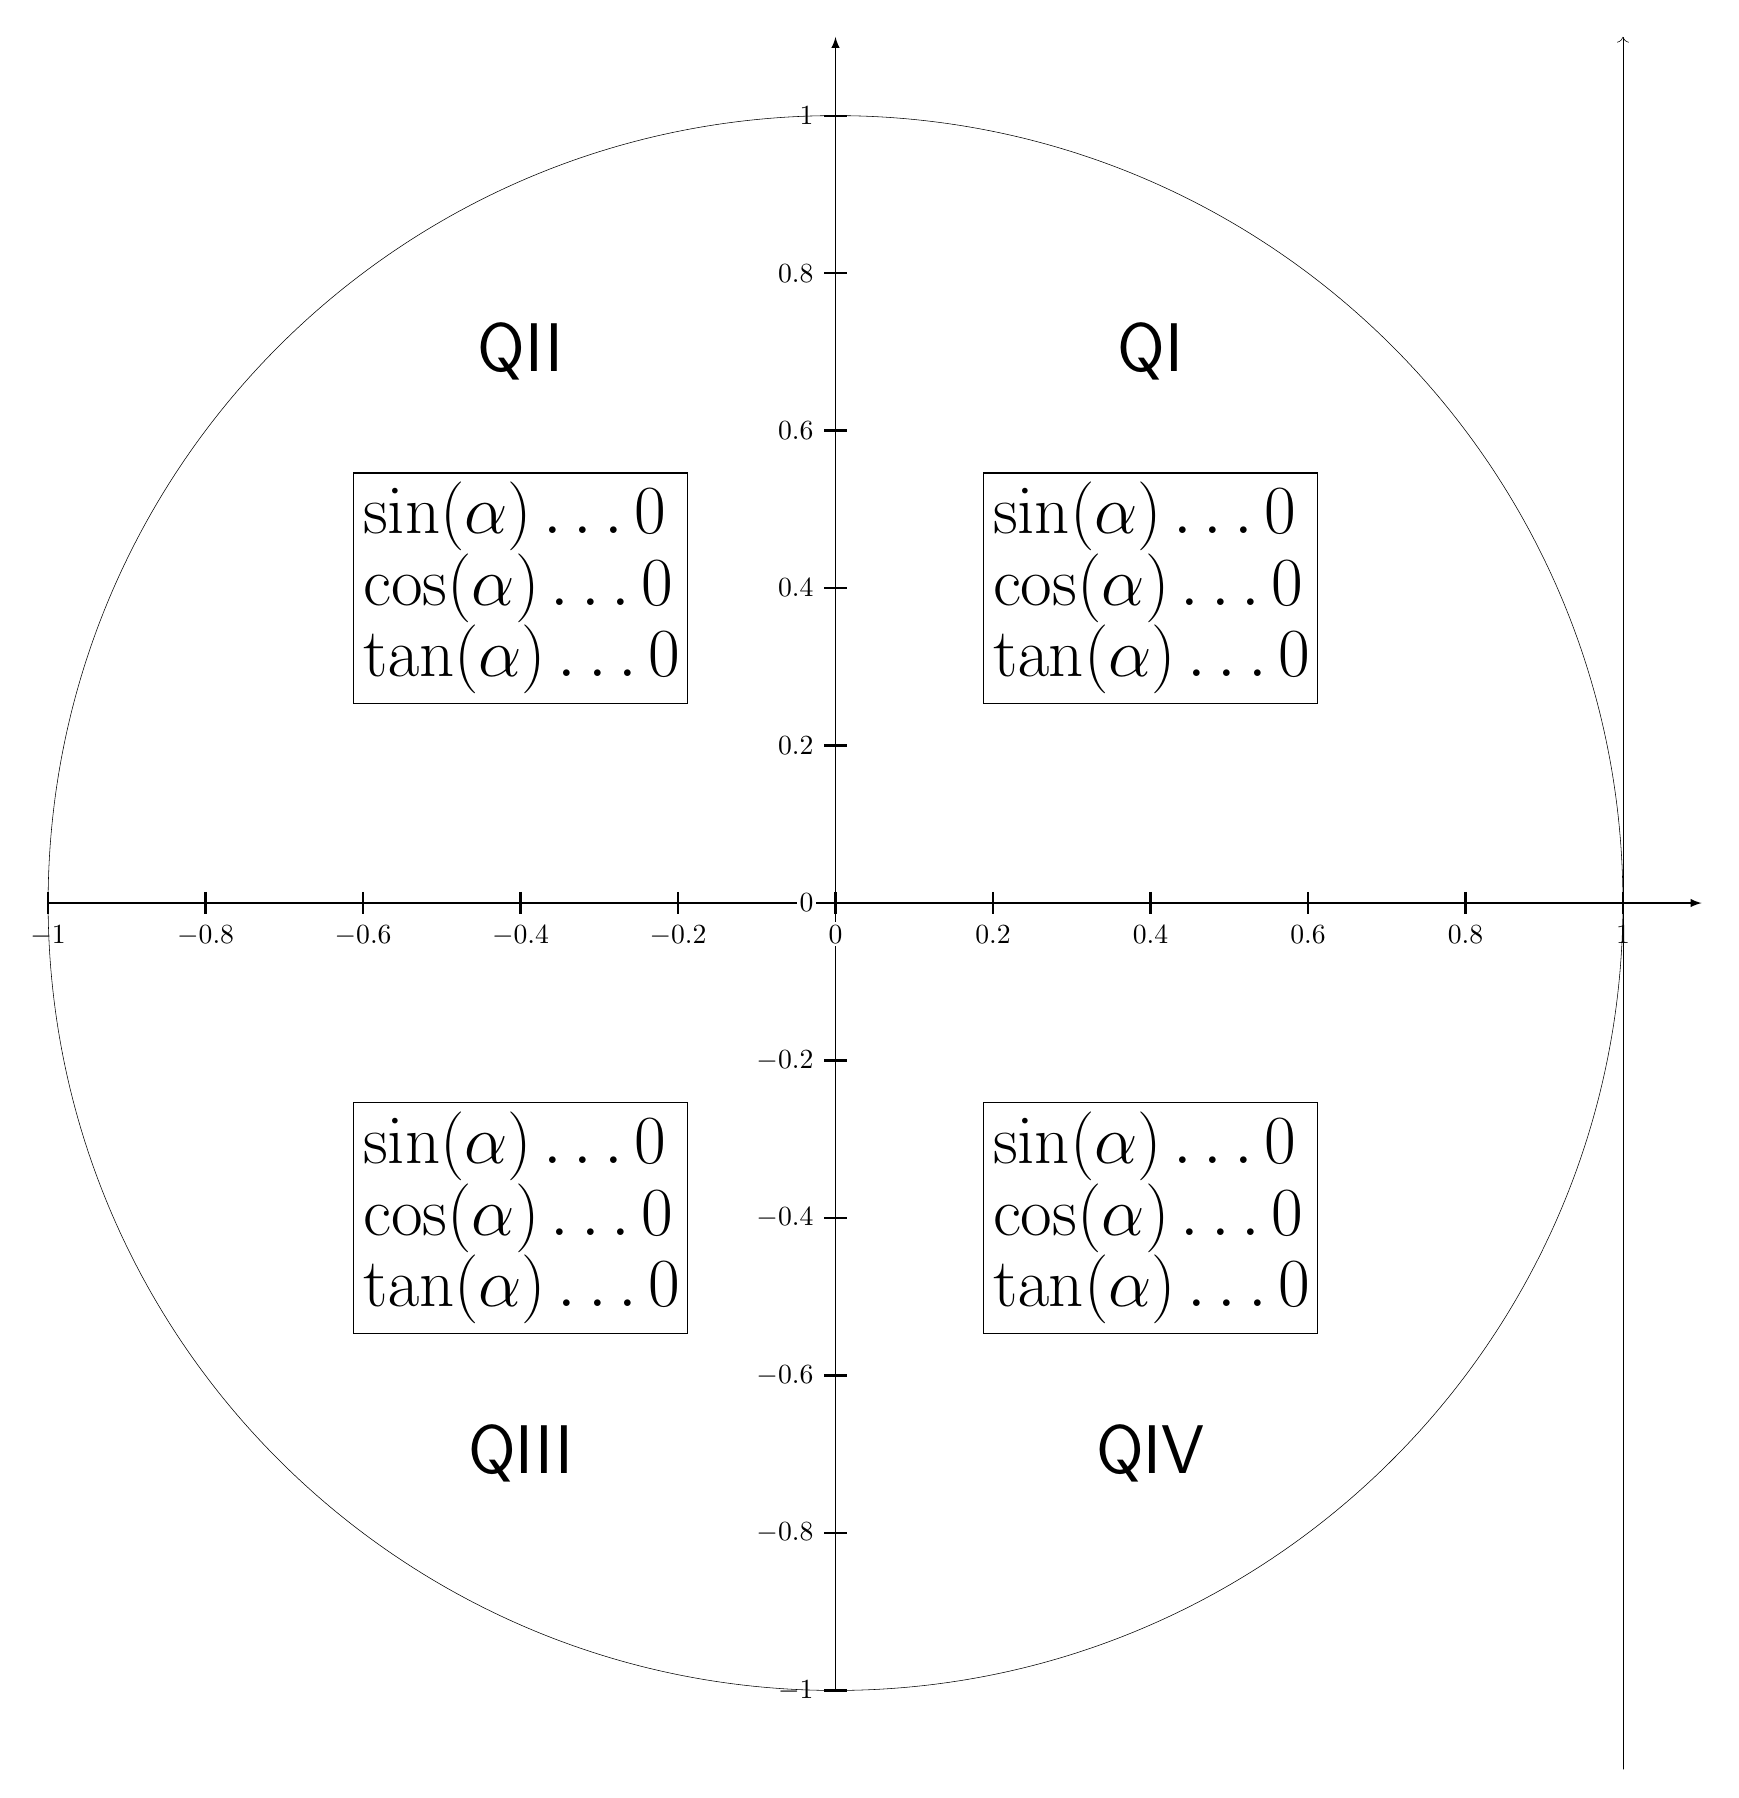
\begin{tikzpicture}[scale=2]
   \tkzInit[xmax=1.,ymax=1.,xmin=-1. ,ymin=-1,xstep=0.2,ystep=0.2]
   \tkzAxeXY[label={}]
   % \begin{scope}[dashed]
   %   \tkzGrid
   % \end{scope}
   \tkzDefPoints{1/1.1/A,1/-1.1/B}
   \tkzDrawSegment[<-](A,B)

   \tkzDefPoints{0/0/O,1/0/A}
   \tkzDrawCircle[color=black](O,A)
\tkzText[draw, text width=4cm](.4,.4){\Huge$\sin(\alpha)\ldots 0$
  $\cos(\alpha)\ldots 0$ $\tan(\alpha)\ldots 0$}
\tkzText[draw, text width=4cm](-.4,.4){\Huge$\sin(\alpha)\ldots 0$
  $\cos(\alpha)\ldots 0$ $\tan(\alpha)\ldots 0$}
\tkzText[draw, text width=4cm](-.4,-.4){\Huge$\sin(\alpha)\ldots 0$
  $\cos(\alpha)\ldots 0$ $\tan(\alpha)\ldots 0$}
\tkzText[draw, text width=4cm](.4,-.4){\Huge$\sin(\alpha)\ldots 0$
  $\cos(\alpha)\ldots 0$ $\tan(\alpha)\ldots 0$}
\tkzText(.4,.7){\Huge QI}

\tkzText(-.4,.7){\Huge QII}
\tkzText(-.4,-.7){\Huge QIII}
\tkzText(.4,-.7){\Huge QIV}

\end{tikzpicture}
\end{document}
